\chapter{The creation of a PCG-based Hybrid Game}
\label{sec:dev}
Creating a hybrid game using PCG represents a challenge in both design and technical areas. The hybrid game genre is a recent design space to explore for designers; and even though some experiments (like \textit{False Prophets} and \textit{STARS}) or games (like \textit{XCOM: The Board Game}) already exist, exploring this concept means raising many questions about how the digital device should be integrated, and what play experience is enabled by the support of PCG.

The thought process of \textit{Archipelago}'s design and development must be thoroughly explained. Describing the game design procedure prototype by prototype would not be relevant in the case of a hybrid game like \textit{Archipelago}. Instead, the origins and evolutions of what are thought to be the crucial aspects of \textit{Archipelago} related to the problem statement should be detailed.

The following section will start describing the development process \textit{Archipelago} by identifying the challenges that appeared when thinking about hybrid games using PCG. To follow, different aspects of the game's design will be described in order to clearly understand the purpose of \textit{Archipelago}. Each aspect of the game analysed in this section is intended to provide results both on the design and technical aspects of its creation in later sections of the report.

The final part of this chapter, on the other hand,  will follow the development of the application in a linear way, following how and when the different choices for the application were implemented based on the design choices that were made.
\section{Ideation and Game Concept Choice}
Brainstorming over the concept of a hybrid game is already a challenge in itself. Because of the experimental nature of the project and the time in which the game must be created, focusing on the key challenges that are expected, and reveal new ones all along the process was a natural direction to follow.
\subsection{Identifying the challenges}
In order to explore the use of PCG in tabletop games, it was important to brainstorm around what PCG could bring to the genre, and what are the pitfalls of such a combination. Based on the previously established framework, the main ideas can be pointed out (see appendix \ref{fig:brainstorm1}).
\begin{itemize}
\item A hybrid game is made of both digital and analogue components. The first challenge to keep in mind is that both types of components must be used for a good reason. In other words, the choice for the core mechanics must prove that the contribution of analogue components could not be simulated on a computer; the same perspective is adopted for the digital part of the game, which cannot be replaced by any kind of analogue components.  
\item Another concern is to preserve the tabletop game experience, and not denature it because of hybridization. Therefore, the core concept of the game should stress out the particular element constituting such an experience. As previously stated, tabletop games cannot be reduced to the use of components or the fact they are played on a table. The social dimension of tabletop games is one of the key elements to stress out in order to make the analogue part of the game relevant.
\item Creating a hybrid game means comprehensively implementing a digital device to enhance the traditional game mechanics. \textit{Enhancing} does not mean creating \textit{better} mechanics. But using a digital component in the game must "have a clear added value" (De Boer and Lamers, 2004, p.443) \cite{chap:aug}. This brings another challenge which is tied to those above mentioned. The use of the digital component must bring something new to the tabletop gameplay experience, and the players should be the first ones to notice.
\item Moreover, the concept of "replayability" (Smith et al., 2011, p.2) \cite{pdf:pcgbased} inherent to PCG-based game design must be illustrated. The focus here is to make this concept visible by the players, who should understand that the game they are playing is flexible enough so that they could replay the game without facing the same situations several times.
\item The concept of "player control" (both "direct" and "indirect") \cite{pdf:pcgbased} over the procedurally generated content - linked to PCG-based game design - is also one that should be experimented with thanks to hybrid games. It is one of the enhancement that was hoped to be achieved and tested throughout the project. It has been previously stated that player control is an interesting contribution to PCG-based game design, as it triggers an uncertainty related to a sufficiently varied creation of content. The players should feel that they have a certain control over the content generation, but still be surprised by unexpected outcomes.
\item This leads to "adaptability" \cite{pdf:pcgbased}. The adaptation of the content to the player's actions in the game would be one of the crucial aspects of the experiment because it shows one aspect that is hard to recreate in tabletop games without the use of computing (though certainly not impossible). However, by using a large number of parameters to feed the PCG algorithm, the content generation would provide a variety that is in this case definitely impossible to reproduce with only analogue components.
\item The theme must support the tabletop game experience, as well as be coherent with the use of PCG.
\item Finally and to stress out the core tabletop gameplay, it is necessary to be cautious about how intrusive the application is in the game. One of the challenge while designing the game would be to provide enough information to the digital device so that a sufficiently varied content could be generated without requesting too many inputs from the players. More generally, avoiding \textit{algorithm specific inputs} that go directly as parameters to the algorithm in order to customize it to the next state of generation was necessary. Therefore, they should be well hidden  behind the game mechanics.
\end{itemize}
These challenges were the main ones that the project should cover. To do so first requires finding a game concept to build upon.
\subsection{Finding a concept meeting the challenges}
Following the principles previously stated, a first game concept based on a core loop had to be found. The different patterns have to support each other, put the players in front of dilemmas and be blended in a core loop on which the whole gameplay is based on.
\subsubsection{A PCG-based design pattern}
\begin{figure}[!ht]
    \centering
    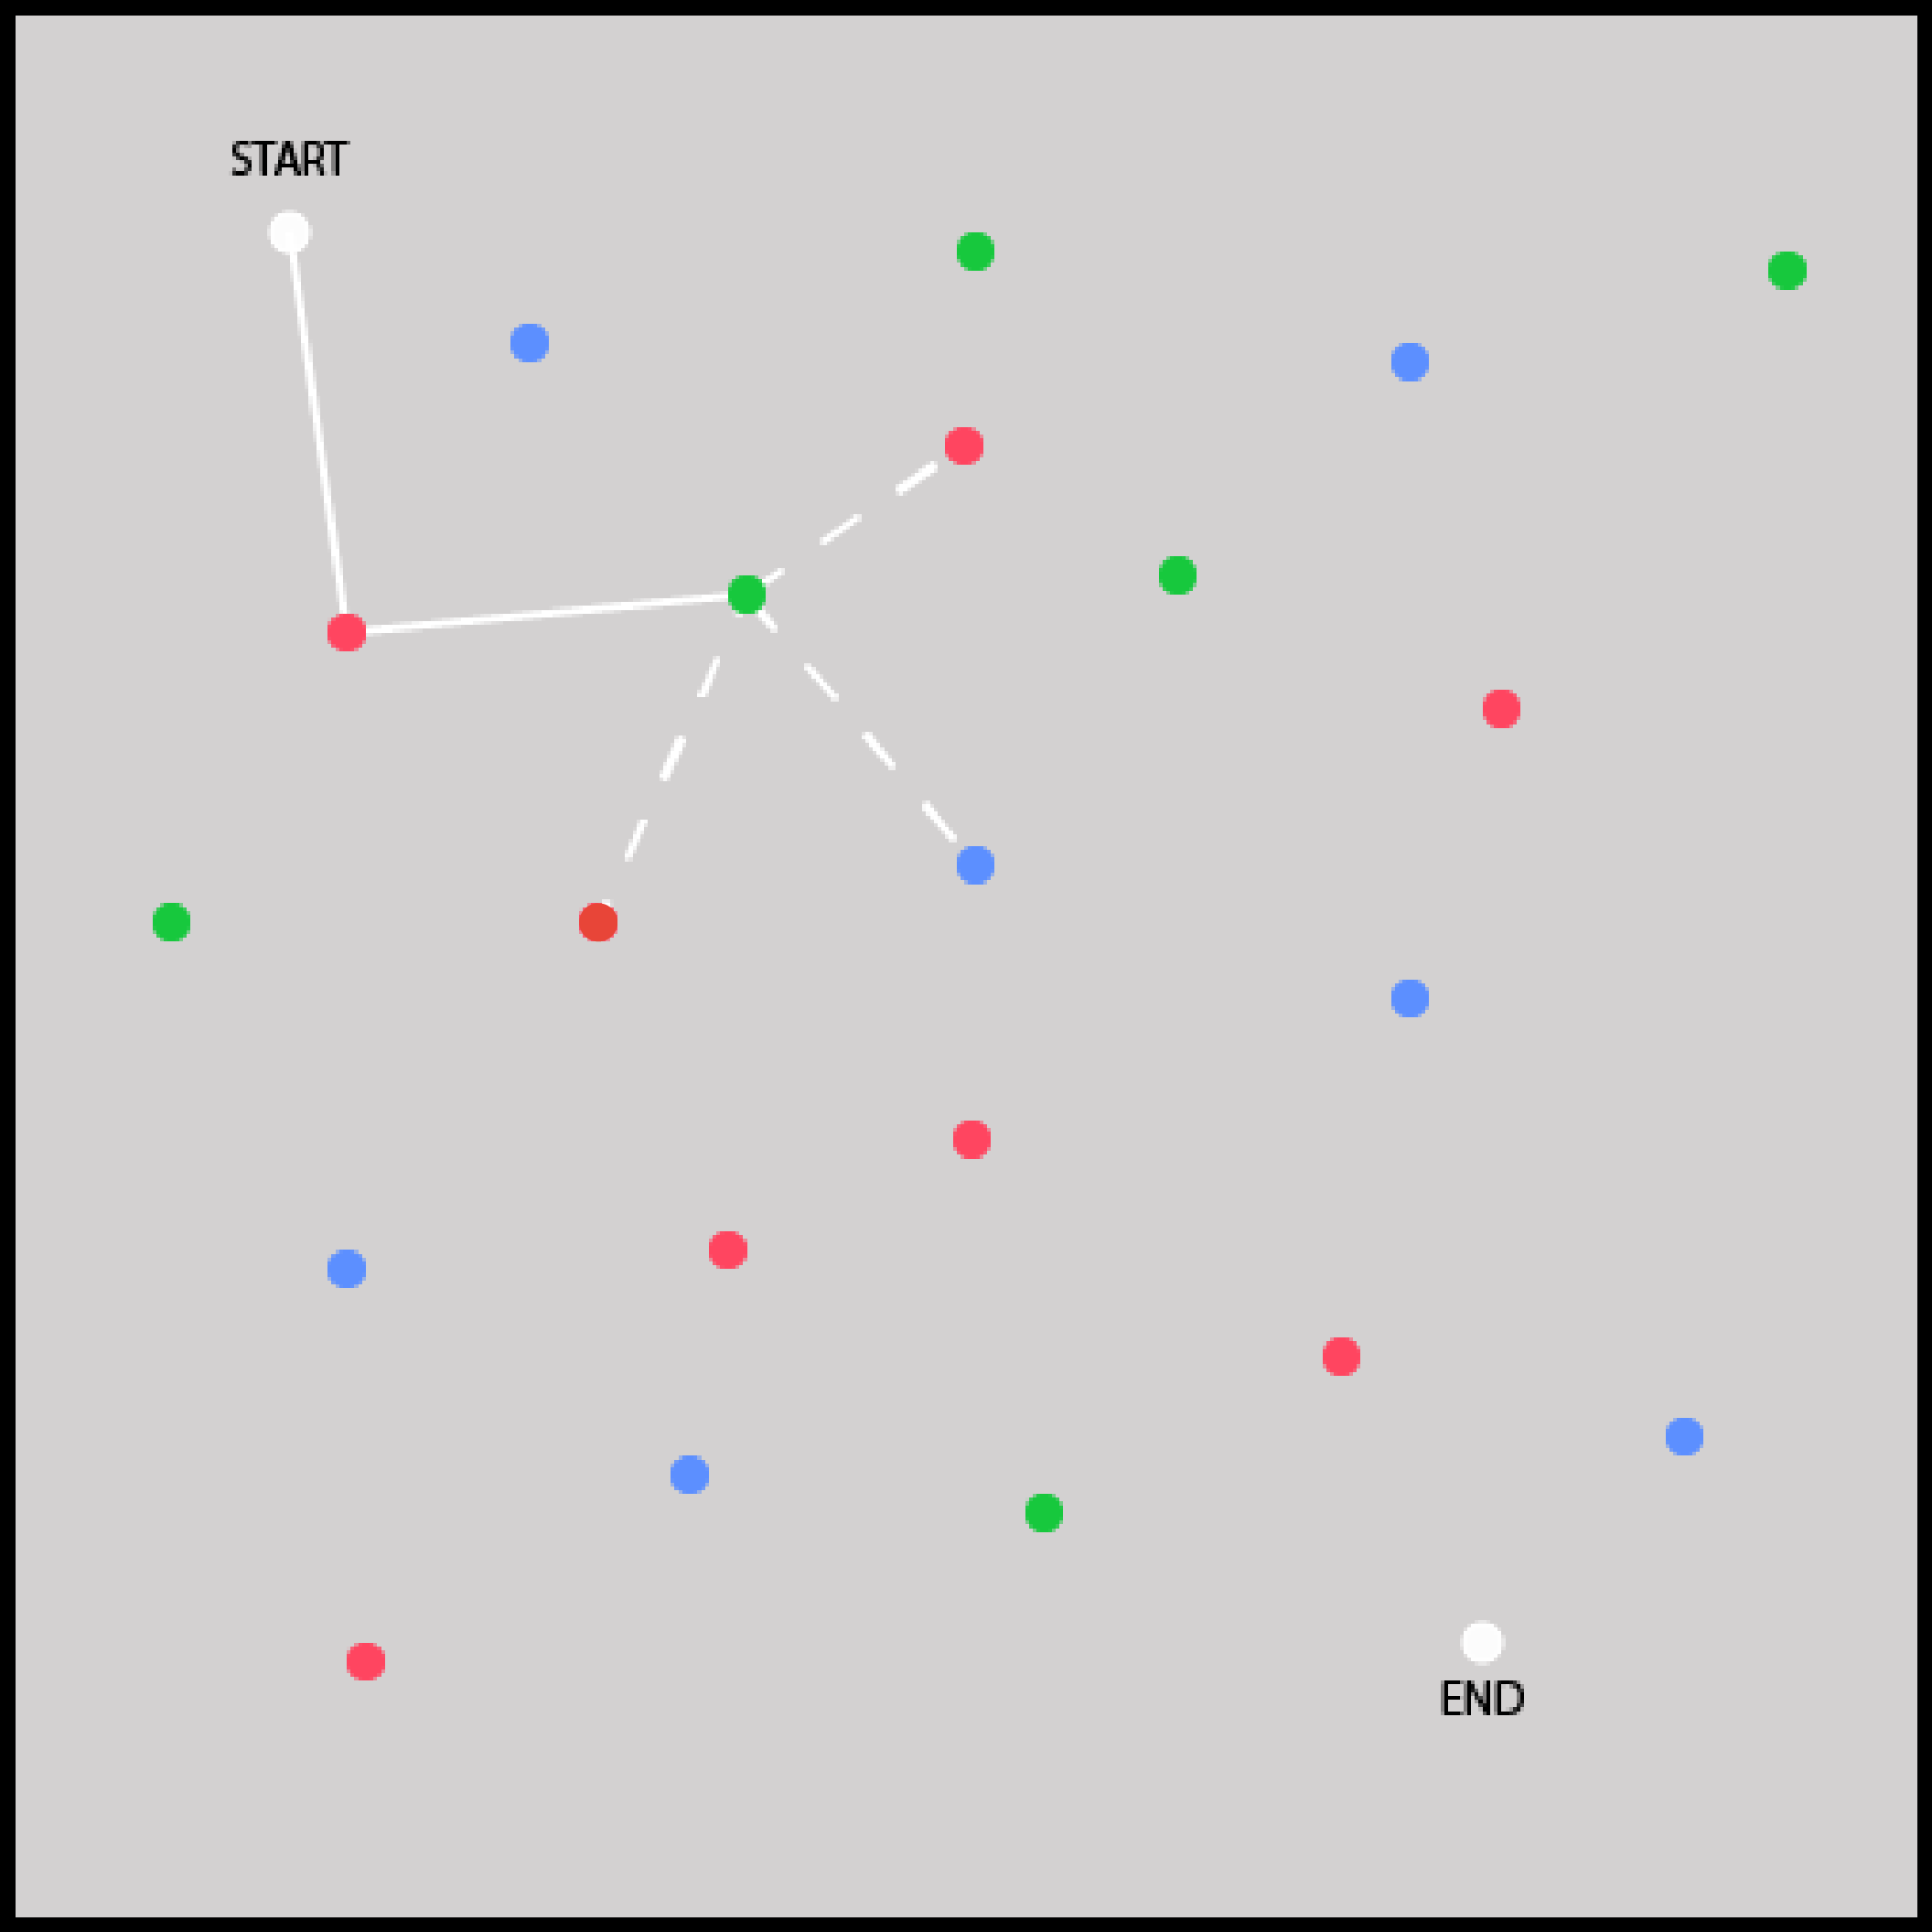
\includegraphics[scale=0.4]{Images/protomap.png}
    \caption{First map mock-up used to communicate the basic concept to the team. The nodes of different colours show the various types of locations accessible. The dotted line shows the nodes that can be reached in one move, and the full line shows the already visited nodes.}
    \label{fig:map}
\end{figure}
The first design pattern that was considered  was the \textit{Node exploration}. The player would need to explore nodes displayed on a map towards a final destination (see figure \ref{fig:map}). Examples of such mechanic can be found in \textit{FTL: Faster Than Light} \cite{game:ftl} or \textit{Out There} (Mi-Clos Studio, 2014) \cite{game:outthere}. The players would have to travel from node to node on the digital device supporting  \textit{Archipelago}'s gameplay, and progress thanks to the outcomes procedurally generated. This pattern has several benefits, and also several implications. 

First of all, the node's content varies depending on the game but is often based on a risk versus reward concept. In \textit{FTL: Faster Than Light} \cite{game:ftl}, the nodes contain events which all have different forms, but in general the player has to make a choice in front of a dilemma (e.g. fight or flee). It is sometimes a good idea to run away instead of trying to get the reward because the risk of a situation is sometimes hard to evaluate. In \textit{Out There} \cite{game:outthere} the nodes contain a star system with planets to explore to extract resources. It is sometimes better to save fuel to visit more locations instead of exploiting all the planets that can be found and run out of fuel - and lose the game.  

These two examples illustrate that the player has to foresee the potential reward the node's content can provide, and balance it with the necessary risk to take in order to access it. The crucial part of this idea is to be found in the \textit{necessity} of the risk, and the \textit{possibility} of getting a reward. The outcomes depend on the player's choices at each node. Generally, the difficulty of the choice that the players have to make in PCG-based games enables the very specific pleasure - and sometimes frustration - of randomness. However, this kind of risk versus reward play experience is very frequently used in tabletop games (often reproduced with a die roll). For this reason, another value should be added to this pattern, thanks to the use of PCG to create nodes and content impossible to simulate with analogue components. This would be included in the scope of several prototypes.

This pattern naturally fits into a gameplay loop. It is a mandatory action that can overthrow a situation if the risk taken by the player is too big - in the case the player is unprepared, or if the risk was not realistically estimated. Finally, mechanics based on this pattern using PCG are challenging to design because of the many possibilities that the players can be confronted to. This would provide an interesting base to experiment with, in order to create a new enjoyable way of experiencing board games.
\subsubsection{Board Game mechanics}
\begin{figure}[!ht]
    \centering
    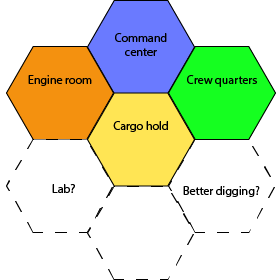
\includegraphics[scale=0.5]{Images/Base.png}
    \caption{Early mock-up describing the tiled structure of the base. Each dotted hexagon represents a possible new upgrade of the base.}
    \label{fig:base}
\end{figure}
The \textit{Base Management} pattern is the next one that was chosen to create the analogue part of \textit{Archipelago}. The term \textit{base} here refers to the central part of the game, that the players would use to travel from one node to the other. This pattern is closer to tabletop game mechanics, where the players use the different resources available to progress through the game. As an example, the game \textit{Agricola} (Rosenberg, 2007) \cite{game:agri} illustrates this mechanic in various ways: the players need to improve their resources collecting capacity in order to manage their farm and their family. This creates a progression based on the player's ability to manage resources correctly in order to produce more during the later turns in the game. In \textit{Archipelago}, the resources have different uses and origins. On the same principle, the various ways in which the base can be upgraded provides a variety of gameplay and strategies, thus enforcing the "replayability" of the game.

By combining those two design patterns, \textit{Archipelago} merges mechanics specific to PCG-based games with others that can well be based on a game board, although not specific to the tabletop genre. An additional element from the tabletop game definition was then required to make of physicality a crucial aspect of the game, and justify its \textit{hybrid game} denomination.

\subsubsection{A PCG-based collaborative board game}

Designing \textit{Archipelago} as a collaborative game was a solution to make a successful combination of a board game mechanic based on tiles, and exploration of procedurally generated locations. One single base is shared by all the players thus emphasizing the social dimension of tabletop games. This is one of the things that make the board irreplaceable in the case of Archipelago. The board provides an interface around which players gather and plan the management of the base and the allocation of the necessary resources.

The collaboration also enhances the PCG-based mechanics of the game in an original way. Indeed, games using this mechanic usually leave their player alone when evaluating the risk of performing an action or not. The fact that a player is on her own when taking decision enables a very special experience - a mix of relief and sudden joy that can be followed very closely by frustration or regret. With \textit{Archipelago}, this special experience should be preserved, but this time, the players would have to take the decisions together. This different approach also brings another kind of flavour to hybrid games, and it was hoped that the discussions that would take place before performing the events would provide a particular experience, confronting the players to the failure - or success - based on a team member's decision.

The combination of those patterns was the base of the core loop (see figure \ref{fig:loop}). The players would have to collaborate managing their base using the resources found during the event exploration. The events would be procedurally generated and only occur on the digital device. Building over such an abstract game concept required another brainstorm session to explore the possibilities offered by such mechanic, and exploit the digital component using PCG (see appendix \ref{fig:brainstorm2}). The inspirations found after the brainstorm session gave directions to explore potential hybrid game specific experiences.
\begin{figure}[!ht]
    \centering
    \includegraphics[scale=0.5]{Images/Core_loop.png}
    \caption{The core loop and the three different steps dividing one turn.}
    \label{fig:loop}
\end{figure}
\section{Designing \textit{Archipelago}}
As mentioned earlier, the PCG integration in hybrid games on a design point of view is explored via prototypes. Based on the prototyping methods and playtest results analysis explained in section \ref{sec:proto}, the game evolved towards a final state which encompasses all the different mechanics used to prove the interest of using PCG in a hybrid game. Instead of describing the different steps of the development one by one, the most crucial aspects of the game supporting the research purpose and the principles behind their evolution will be described in this section.  
\subsection{Early prototyping}
Testing the core mechanics is necessary before moving on to the implementation of the digital device and the PCG. The purpose of this prototype is to experiment the core loop as well as the first basic mechanics around which the game would be built and communicate this concept to the team.
\subsubsection{First iteration}
\begin{figure}[!ht]
    \centering
    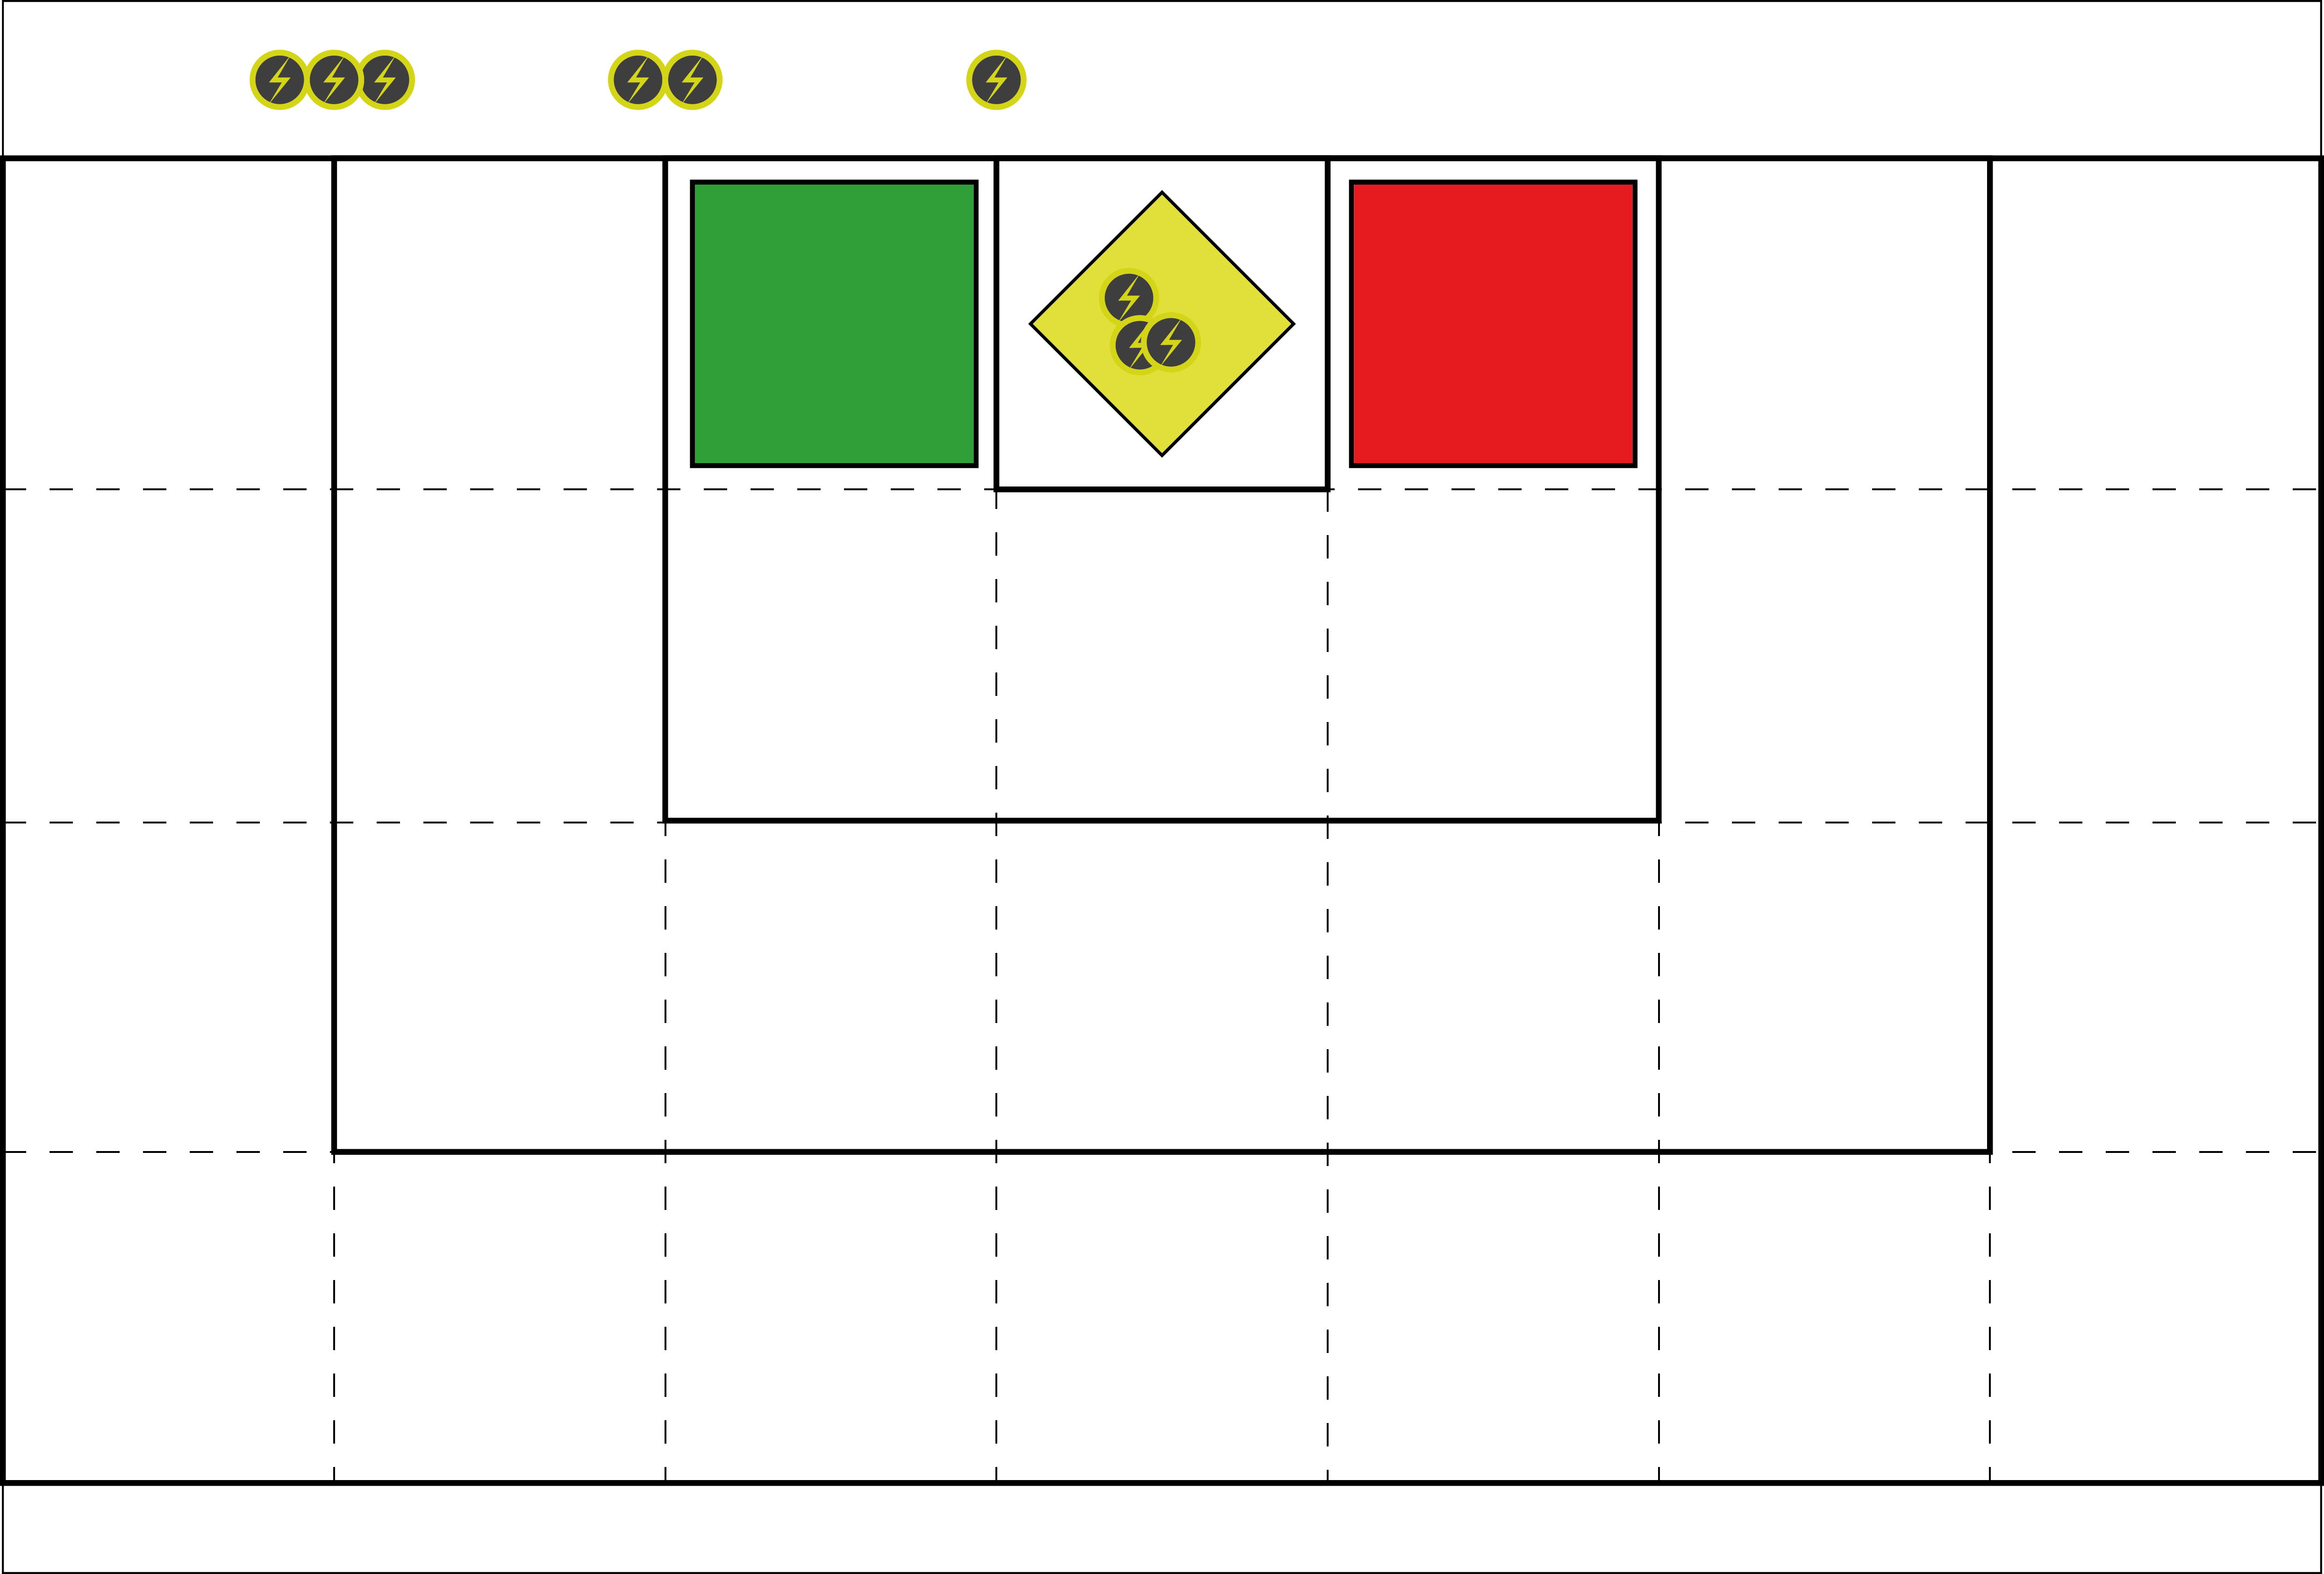
\includegraphics[scale=0.5]{Images/Board1.png}
    \caption{A representation of the base used in the first prototype.}
    \label{fig:base1}
\end{figure}
Based on Lim et al.'s framework to create relevant prototypes, the first iteration of \textit{Archipelago} can be described by its main properties.

Being the first version to be tested by players external to the team, the application using PCG is not part of the prototype (see figure \ref{fig:base1}). Therefore, paper and dice compose the \textit{Material}. The paper is used for the representation of the base on the game's board, and more generally all the different analogue components like tiles and tokens; the dice are used to simulate the PCG part. 

It has a low-fidelity \textit{Resolution}: the representation of the base is still very abstract and the digital component of the game only simulated. There is also no real theme attached to it. 

The \textit{Scope} includes several purposes: testing how the base should be represented on the board and how it should be managed was the first one. Experimenting a basic resource system based on collaboration was also important to provide a basic idea of how the game should work. Finally, it was also vital to know when the digital component should be used in the game.

At this stage, the mechanics of the prototype already contain several elements that are still in the final version (sometimes in a different manner). Refer to figure \ref{fig:base} for each description given below:
\begin{itemize}
\item The base is divided into squares, each square being a space where building a room is possible. The different spaces are distributed in \textit{Construction Zones}, which have to be unlocked in order to extend the available construction space. To unlock a zone, the players have to power the \textit{Core} with \textit{Energy} tokens. The amount of \textit{Energy} tokens required to access a construction zone is indicated at the limit between the two zones.
\item The \textit{Cargo Hold} tile limits the \textit{Scrap} (used for construction) that players can have to 2 tokens per \textit{Cargo Hold} tile.
\item The \textit{Crew Quarters} limits the \textit{Crew members} that players can have to 2 tokens per \textit{Crew Quarters} tile.
\item \textit{Scrap} tokens, \textit{Crew member} tokens and \textit{Energy} tokens are gathered thanks to the \textit{Exploration Room}. To start gathering, the players assign a \textit{Crew member} to the \textit{Exploration Room} and roll a die. Assigning two \textit{Crew member} tokens (the maximum the room can contain) provides a second die roll (see figure \ref{fig:Dicetable}). Gathering can only be done at the end of the turn.
\begin{figure}[!ht]
    \centering
    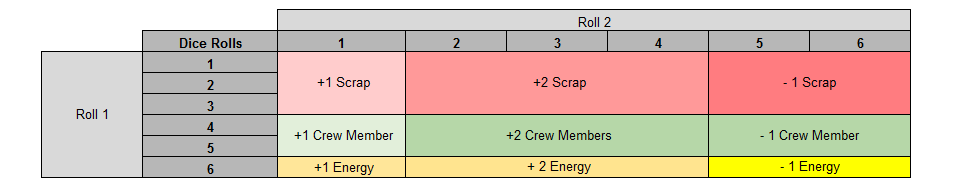
\includegraphics[scale=0.6]{Images/DiceProto1.png}
    \caption{Table representing the results of the dice rolls. One die only gives access to the leftmost column of results. A second die gives access to better rewards, but there is a risk of losing resources. There is still a chance to get a standard reward with two dice, so the risk is not necessarily worth the reward.}
    \label{fig:Dicetable}
\end{figure}
\end{itemize}
\subsubsection{Feedback from early playtests}
Feedback from the first testers showed that even with abstract components, the flow of the game provides a sufficiently good base for discussion. According to playtesters, dividing the board into \textit{Construction Zones} is also an interesting mechanic in itself. But it appeared several times that the players were stuck with not enough resources to play.

The randomness of the results (due to the use of dice) also showed the problem of engagement in the game. The players were easily frustrated to lose resources because of a simple dice roll. This emphasizes the notion of player control tied to PCG-based game design. On the other hand, using more than one parameter proved that the players need to feel their influence on the generation of the rewards: it happened that one player tried to convince the others that using two dice would be more efficient whereas the others thought that the risk to lose a reward was too big. Later prototypes also based on dice and paper proved that giving the possibility to influence (increasing or decreasing) the chance of getting a negative outcome could strengthen the feeling of control. This enabled more engaging discussions between the players. However, the level of abstraction showed problems of frustration.


To encourage the players to show more engagement in the game and to allow for more interesting collaboration, a specialization mechanic was built in the later prototypes. This mechanic is an important aspect of \textit{Archipelago} and will be described in a later section. 
 
Finally, this prototype gave a good idea of how the flow of the game should be. It was decided to build the work over this core loop to start implementing the PCG and the digital device in the game.

Following the bases of the first prototype, a turn in \textit{Archipelago} is divided into two different phases:
\begin{labeling}{Management Phase}
\item[\textbf{Management Phase}] The phase during which the players discuss and allocate the different resources in the most efficient way. This phase is based on the physical components, gathering the players around the board and using the game pieces.
\item[\textbf{Exploration Phase}] After the management phase, the players choose an island to explore on the device. This island contains locations to visit, and si\-tuations to overcome. The choices made by the players condition the amount and nature of resources they are getting. The PCG would generate the island layout, the situation that the players have to face, the options they have and finally the outcome of the event.
\end{labeling}
As previously mentioned, one of the challenges of making \textit{Archipelago} was to make both digital and analogue aspects of the game support each other without interfering play as well as being essential in the game. Another important aspect justifying the purpose of this experimental game was to bring an added value thanks to the use of a digital component. PCG should bring this added value in various ways, and still be coherent with the game system and theme.
\subsection{Using theme and narrative}
In \textit{Archipelago}, the players have been sent by the King of their homeland to explore a newly discovered archipelago of floating islands. They are commanding a flying castle that is powered by a crystal emitting energy. The castle is composed of rooms that each have several functions in the game (both in the management phase and the exploration phase). These rooms range from \textit{Mining Guild} allowing the players to gather the required material for construction; to \textit{Mechanic's Workshop} to repair the rooms that are damaged during the exploration phase. The players have to fly from one island to the other in order to reach the final island on the map and finish the game. Islands are composed of different locations, which are generally filled with magic: magic crystals are scattered around the archipelago and with time created strange effects.

The archipelago is inhabited, though, and the players will have to confront the different factions, sometimes by  allying; other times by betraying. The relation with the factions influences the outcomes in various ways, modifying the number of resources that players gain, and affecting the game's difficulty. The events then become more and more dangerous as the players progress and acquire a reputation in the archipelago.

The world of \textit{Archipelago} takes place in a \textit{Fantasy} based world during an industrial era. The different countries have an increasing need for resources and the Archipelago is an \textit{El Dorado} for explorers on a quest for riches. The theme condenses the different aspect experimented by the game. Although it does not exactly follow a setting that is known to every player, it uses a template of references that makes each aspect of the game identifiable. By situating the game in an unexplored place, finding a large variety of procedurally generated islands feels natural. The players are the commanders of the flying castle, and all the resources they use are explained in the management phase have been made coherent with the theme. For example, the fact that the islands are floating is the consequence of the crystals scattered around the archipelago. The flying castle also floats thanks to these crystals, and the players must power it with crystal parts that they find on the islands. 

The name of the different rooms and upgrades also follow the theme, so that the players can rapidly have a general idea of what they are used for before learning by playing or reading the rules. It is important to know that the core concept and mechanics were not chosen because of the theme, rather the opposite. Various ideas were experimented and this one was chosen at the very end of ideation phase. Therefore, \textit{Archipelago} was not constructed with the specific purpose of exploring narrative possibilities in a board game. However, it is true that the game should prove that PCG enables the possibility of supporting hybrid mechanics thanks to variations in the narrative. The prototyping efforts should then cover this aspect to analyse the contribution of PCG in the support of mechanics by the theme.
\subsection{Specialization and collaboration to support a tabletop play experience}
\textit{Archipelago} offers a collaborative experience, based on the player's specialization in different areas of expertise. Following the definition established previously, \textit{collaboration} means that all the players share the same goal: reaching the final island and avoiding to lose all the power contained in the castle's crystal. All their actions must follow this purpose, and they must leave to the other players what they cannot do themselves. An original approach was imagined in the case of \textit{Archipelago}.
\subsubsection{Constructed Specialization}
Cooperative or Collaborative mechanics in games often follow a standard rule. The players choose one role that they will keep until the end of the game. This role comes with specific aptitudes which support each other, thus outlining the team dynamic in the game (see section \ref{sec:xcom} for an example). In general, the roles are interconnected, and one player cannot fully exploit her skill without collaborating with another player.

In \textit{Archipelago}, the specialization was designed to be constructed by the players themselves. The specializations are given names related to the theme:
\begin{itemize}
\item The Chief Miner is responsible of the collection of the material necessary to build the rooms in the castle. 
\item The Alchemist sends crew members in locations during events to collect the alchemical components required to upgrade a room to a more efficient one of the same type.
\item The Mechanic repairs the rooms that were damaged during events.
\item The Priest heals the \textit{Crew Members} that were injured during events.
\end{itemize}
Originally, the specialization was based on the distribution of roles to the different players following a classic concept. The players then had specific actions to perform that the others could not do. After a few prototypes using this mechanic, though, it was observed that the mechanics of construction and room building was not a sufficient support for discussions, and some players were basically watching the others playing. Sometimes, a player had nothing to do during a turn, because her role was not required at that moment. Therefore, the model was changed to allow the players to \textit{construct} the specialization themselves, by choosing which player would take on a role along the game.

It seemed that this mechanic would also fit nicely in a PCG-based game. As the outcome are procedurally generated, the strategies for specializing should vary from one game to the other. In a constructed collaboration system, there is nothing encouraging the players for choosing a specific role over the others. However, specializing will offer a variety of bonuses that players must split as they cannot have them all at once. This is why the specialization is \textit{constructed}. The roles are not attributed according to a game rule, but because players must feel the need to do it. Therefore, some mechanics have been designed specifically to encourage the collaboration and emphasize the need for collaboration.
\subsubsection{Encouraging Collaboration} 
An important mechanic that has followed the game from its first iteration was the attribution of \textit{Crew Members} to a specific player. This means that all players have a team of \textit{Crew Members} that must be assigned to perform all the actions in the castle as well as during the events in the exploration phase (thus acting as action points). \textit{Crew Members} are the only resource that is not shared by the players.

This is how \textit{Archipelago} forces the players to efficiently split the tasks. All the other resources are shared, though limited. \textit{Crew Members} can be gained after performing an event, and their attribution to a player is decided by the team. It is important to notice that the \textit{Crew Members} can be either injured (and unavailable until they are healed by the priest), or killed. Players must have at least one \textit{Crew Member} under their command. If a player loses all her \textit{Crew Members}, another player must give one of hers. If there are less \textit{Crew Members} in the castle than players, the game is lost.

Observations during playtests showed another problem that was unexpected. When testing with players who had different levels of experience with tabletop gameplay, it happened often that some players would take a role as \textit{leader} and took all the decisions for the team. The specialization system intended for \textit{Archipelago} was not supposed to follow this line. As explained before, the players should have their authority in their field of expertise and must feel that they are important. Although sometimes this problem could be attributed to the engagement of some players who were less involved than others, this problem should not happen in the final version of the game. It was expected that offering enough variety and unexpected outcomes with PCG should tackle this problem.
\subsection{Enhancing Replayability} 
The first aspect generally cited to enhance play with a PCG-based game design is replayability, which is the idea of replaying the game without facing the same situations. The replayability of \textit{Archipelago} is supported by one of its most crucial aspect, which is to exploit PCG to generate the income of resources supporting the collaborative tabletop gameplay. The design of the event generation system was then an important part of the development and the ideas behind its evolution should be explained.
\subsubsection{An infinite number of events}
After simulating the event generation system with dice, the first iteration of the event generation system was included in the \textit{Scope} of another prototype. As observed during early prototyping, the number and quality of parameters selected to create those events and their outcomes were a crucial aspect of the design. The prototype should then introduce those parameters both to the players and to the development team. Prototyping the event generation should then help to manifest two main design problems:
\begin{itemize}
\item Finding the right number of parameters to use in order to generate a content in which the patterns of the event generation system would not be recognized by the players.
\item The parameters must be intuitive for the players so that their decisions are based on the ones that they can recognize; it must also be technically coherent so that the data could be reused for generating consistent content based on the players' actions.
\end{itemize}
This is not the first iteration implementing a digital device in the flow of the game: an iteration of the procedurally generated archipelago map layout had been tested along with the dice mechanic to further experiment on the flow of the game (see appendix \ref{fig:gameflow}). However, it was the earliest prototype using digital components in its \textit{Material}, to generate text-based events.

In \textit{Archipelago}, the events are generated every time the players enter an island and have several properties. First, a text describing the situation is generated. This text depends on the \textit{location type} that the players have selected on the island. The players have several \textit{options} to face this situation. These options are only accessible to the players if they possess the required \textit{conditions} (i.e. the necessary resources or upgrades in the castle). The text describing the options is also procedurally generated. After selecting an option, a calculation is made to determine if the event was successful or not. The amount of resources collected is then determined. 
\subsubsection{First iteration of the event system}
The first event generation system simply relied on a random percentage based selection of outcomes. So, the interesting part of this prototype is not to be found in its technical aspect, but in the exploration of the different parameters needed to generate coherent text-based events:
\begin{labeling}{Class or Priority}
\item[\textbf{Event Type}] Three classes of events which are guidelines for their content.
\begin{itemize}
\item \textit{Gather} is related to the extraction of \textit{Scrap} (Construction Material) used to build new rooms in the castle.
\item \textit{Research} contain events linked to resources  used to merge the different rooms so they are more valuable.
\item \textit{Diplomacy} handles the encounters with the factions, and is a premise of what would become the later \textit{Faction System}.
\end{itemize}
\item[\textbf{Option Class}] The options available to the players to solve the events presented to him are divided into \textit{Basic}, \textit{Second} and \textit{Third}. The Events always contain options from the two first \textit{Classes}, but the \textit{Third} only has a 50\% chance of appearing. 
\item[\textbf{Risk}] The higher the class is, the better the associated maximum reward is. However, very penalizing outcomes are introduced to counterbalance the rewards.
\end{labeling}
The texts of the different options and outcomes were handwritten. It took a long time to reach a sufficient number of options and outcomes before testing the game. For these reasons, this method was not sufficient to prove the interest of PCG in rapidly generating content to reduce the workload of creators. Also, playtesting showed that the players could recognize the different patterns in the event generation (i.e. options showing several times in a row), thus ruining the replayable aspect of the game. However, this provided a base to work on a more complex event system.
\subsubsection{Prototyping for technical flexibility and narrative coherence}
As observed during playtests of prototypes using the event generation system previously described, the generation of content could not provide enough variety to generate a potentially infinite number of events and transmit that impression to the players. Also, the workload was too high in the prospect of experimenting a sufficient amount of PCG-based game design possibilities. Solving these problems required drastic changes to attain a satisfying amount of coherent results.

A new design method for generating the events was then imagined (see section \ref{sec:eventGeneration} for the technical details).

The \textit{Outcome} is defined when performing the event. This outcome is calculated thanks to the following parameters:
\begin{enumerate}
\item The \textit{Event Type} to select the most likely resource to be collected. In the final version of the game, there are two types of standard events. The \textit{Gathering} events during which the players collect more \textit{Scrap}, and the \textit{Alchemy} events during which the players collect more \textit{Alchemy Points}.
\item The \textit{Condition(s)}, which is the resource(s) that the players use to access the different options available to perform the event. All the events require sending at least one \textit{Crew Member}. This method was used to select which \textit{Specialization} token would affect the reward: only the token of the player(s) sending a \textit{Crew Member} is taken into account.
\item The \textit{Class} of the option selected by the players. 
\end{enumerate}
There are three types of outcomes: success, neutral or failure. The type is defined by the standard risk associated to the \textit{condition}, and the faction controlling the island. 

After an internal test, this method was selected to show the potential of PCG to create a very large number of situations and options for the players during the events. Feedback from playtesters showed that the text also needed to be carefully designed. The text needed to be coherent with the proposed options, and adaptable to a variety of situations. It was composed of different blocks that the digital device organizes in order to create a coherent option, understandable by the players and providing enough information regarding the risk and the potential reward.

Prototyping the text generation was simple. Based on the results from the different playtests, a range of simple parameters were selected:
\begin{labeling}{Faction control}
\item [\textbf{Location Type}] A subdivision of the \textit{Event type} parameter used to calculate the reward. It is used to contextualize the situation.
\item [\textbf{Faction control}] The name of the faction controlling the island.
\item [\textbf{Allegiance}] The relation between the faction and the player.
\end{labeling}

A few tries showed that extra parts were also required to connect the different parts together and make the whole text coherent. For each of these parameters, several text blocks were written on bits of coloured paper (see appendix \ref{fig:paper}). Thanks to the combination of the different chunks of text, it was possible to determine how they should be written to be adaptable in any possible combinations (see figure \ref{fig:textproto}). Simple prototypes using generating texts were built and showed to testers. This gave the basic rules to determine how to generate a coherent text. By having many different blocks of text written on the same model, generating a very large number of flavour text with hardly recognizable patterns became easier. 

\begin{figure}[!ht]
    \centering
    \includegraphics[width=\textwidth]{Images/textProto.png}
    \caption{Examples showing the prototyping method for building the text in the game. All the different combinations are possible. The text adapts itself depending on the content that is generated.}
    \label{fig:textproto}
\end{figure}

The same system was used to generate the option text. This time, however, the text would also be based on the \textit{condition} associated with the option. This would also show the risk associated with the event, the risk depending on the amount of resources used by the players to solve the event (see section \ref{sec:flavour} for the technical details of the flavour text generation). The system was flexible enough so it was possible to experiment various rules to create the events, and increase the quantity of possible combinations. The first new implementation to try was to save data during the events in order to reuse it when the players reach another island later in the game.

The text generation in \textit{Archipelago} is one of the most visible use of the theme to support the gameplay mechanics. By following the different parameters used to create events, the text provides clues about the risk of performing the event and also provides a context to players when performing an action.

While it does not affect the generation of the content strictly related to gameplay (i.e. the outcomes and conditions), testers also positively responded to the division of the \textit{event type} parameter into several smaller locations. They showed more engagement while performing the events and the discussions illustrated this involvement. However, it happened sometimes that the generated was not correctly assembled, or that the rewards did not fit the actual situations. Further testing allowed us to partly solve the problem.
\subsection{Designing player control and adaptability}
In PCG-based game design, adaptability refers to the influence of the players' actions over the generation of content. Although already covered by the event generation system, where the various options that are available to the player determine the outcomes in terms of resources gained or lost, this quality of PCG-based games needed to be emphasized in \textit{Archipelago}. 
\subsubsection{Diplomacy system: another philosophy of event generation}
It has already been mentioned that early prototypes included a \textit{Diplomacy} type of events. However, using diplomacy this way showed an overlap with the other types of events, and it was therefore not interesting for the game to leave it like this. After several prototypes using this parameter to create events, it was decided that diplomacy would be a whole system of mechanics influencing the generation of the events and the gameplay of the whole game. 

The different islands of the Archipelago are inhabited by three different \textit{Factions}:
\begin{itemize}
\item The \textit{Highbournes} are described as humans native of the archipelago. They are a proud people very close to their traditions. They are the first inhabitants of the islands and therefore have been under the magic influence of the crystals for a long time now.
\item The \textit{Nomads} arrived on the Archipelago for various regions of the world. By exchanging with the Highbournes, they have acquired the rudimentary magic skills necessary to create their own transportation means and scavenge the islands for resources. They live in small villages and often confront the Humans that recently populated the archipelago.
\item The \textit{Humans} are the last people who populated the Archipelago. They also arrived from various places of the world, but contrary to the Nomads, they live in large communities based on trade. Their rapid development is the primary cause of tensions between the factions of the archipelago.
\end{itemize}
Every island is controlled by a faction. When players enter an event, they see which faction control the islands by looking at the symbol in the top left corner of the screen on the digital device. As previously explained, the faction controlling the island influences the text generated in the events (both in the options or in the text describing the situation). The factions having different moral and interests, so the approach chosen by the players to resolve an event has consequences. In some specific cases, the actions performed by the players during an event triggers a special event, which is the one that affects the relation between the players and the faction concerned. This special event is also procedurally generated, although more static that a standard event linked to any island. To make it special and recognizable by the players, triggering a special event is made thanks to specific criteria.

\textit{Special events} are events using data stored after the players have previously performed a standard event, thus creating a narrative coherence between the two. Designing those events required a specific method. The special events are only triggered when the players solve a previous event thanks to a \textit{Third} class option. Because the \textit{Third} class option always requires a specific \textit{Specialization} token, it provides theme related information to the PCG algorithm. By combining this with other information like the \textit{Faction} controlling the previous island and the location that was visited during the standard event, it was possible to create a linked event. For example, solving an event thanks to a \textit{Third} class option requiring  alchemist \textit{specialization} in a \textit{Mine} controlled by \textit{Nomads} could generate an event in which the humans followed the team until the next island, asking them \textit{Alchemic} material to help them curing an epidemic ravaging their village. The players generally have several options to solve these special events. Depending on the option chosen, the relation with that faction increases or decreases. Certain choices made during the special events can also affect in certain cases the relation with another faction.

The relation with the faction influencing the PCG in various ways, the diplomacy system has several impact on the gameplay. 
\subsubsection{Influence on the overall experience}
By using the theme of the game and the text generation system, the diplomacy mechanic ties the game's re-playability to the content's adaptability. The variety of the approaches and strategies due to the procedural generation of the islands is reinforced by the fact that some data about the player's inputs are stored by the application and reused to generate the special event. 
In a more technical aspect of the design, changing the relation with the faction is also a way to affect the generation of the events performed during the \textit{Exploration Phase}, and to give a certain feeling of control over the content generation: a player will be more likely to take fewer risks on an island that is controlled by an enemy faction. On the contrary, being allied with a faction makes the events easier to solve.

It is important to notice that the \textit{Special Events} are only triggered after a specific combination of parameters are met, and not every time the players chose the third option class. It is almost impossible for the players to know when a special event is going to be triggered. The Special Events then also enable a surprise element specific to a hybrid game experience. Also by using the narrative elements to show the relation between the triggered event and the previously performed action, the goal was to show that the game world is coherent and evolving around the player. 
\subsection{Making a hybrid game}
Coherently generating events and using the stored data to generate others was an experimental use of PCG in hybrid games. Combining this approach with the mechanics encouraging collaboration was also a way to associate two different types of gameplay to create mechanics that rely both on analogue and digital components. One of the prior concern when creating \textit{Archipelago} was to keep the original tabletop experience intact. Therefore, the application used to create the world map should not be too intrusive in the gameplay. Using the application only once per turn was one of the possible solutions (see figure \ref{fig:wireframe}).

\begin{figure}[!ht]
    \centering
    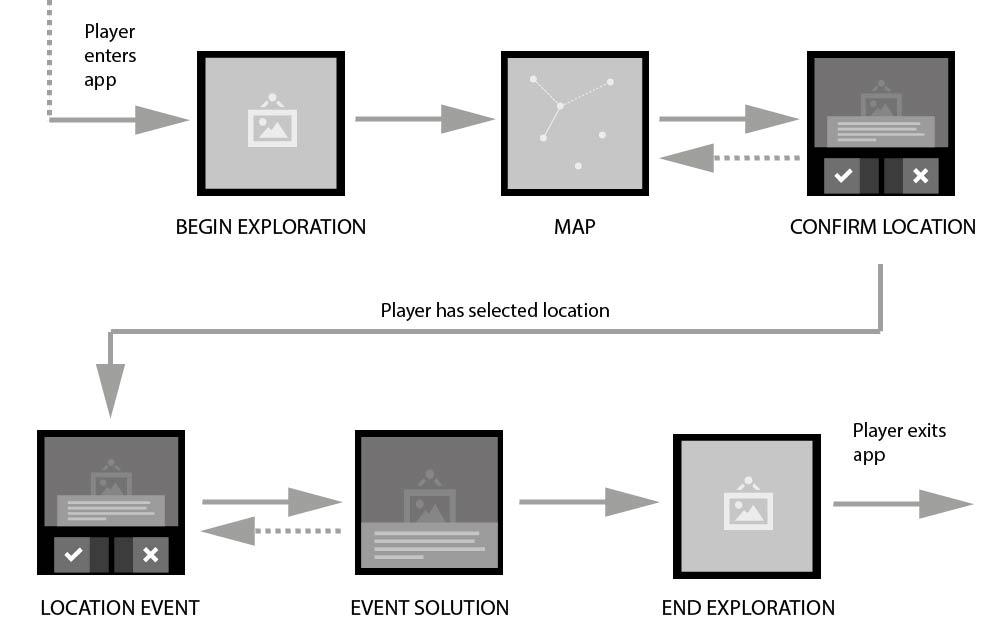
\includegraphics[width=\textwidth]{Images/wire.jpg}
    \caption{Early wireframe showing the different steps that the players would have to go through when using the application.}
    \label{fig:wireframe}
\end{figure}

When playing \textit{Archipelago}, the device is an important element, as without it the players would not get the necessary resources.
Mainly, the function of the application is to contain all the information regarding events, movement, factions and the overall data available within the game. 
When playing the Archipelago, the digital part of the game will provide the players with a layout of the world, i.e. the map with all its islands, and contain all methods of receiving rewards as well as receiving penalties for executed events. It determines which resource the players will receive, what the narrative is (in terms of flavour presented), and it contains the factions (and relation with each of them).

Different ways of representing the various panels used to display the events were tested (see figure \ref{fig:uimockup}). The User Interface had to reuse visual elements from the board as well as fit the overall theme. Different assets were used over the whole process of making the game. It is important to notice though that all the visuals used in the game are placeholders that were used so that the game would be less abstract during playtests. Early tests have shown that the level of abstraction could affect the engagement of the testers. Therefore, all the visuals used in the interface were changed to fit with the theme and contextualize the experience.
\begin{figure}[!ht]
    \centering
    \includegraphics[width=\textwidth]{Images/event.png}
    \caption{Mock-up of the solution retained to display the events in \textit{Archipelago}.}
    \label{fig:uimockup}
\end{figure}

The events in the application, are made to be like cards that the board game would have if there was no application. But by having the digital computing and memory, the diversity of these events are much greater and there is no need for a huge pile of cards and expansion packs to generate different and diverse events. The replayability of the game is then increased by the number of possible events and the order of their occurrence. The rewards received by the players (as well as the penalties) determine the most important rooms to build, how to allocate the resources and which is is the most important specialization to attain first

The application is partially in control over what the players get and what is taken away from them, and given that there is now a memory in place, the possibility to create new content based on previous events is there. The word \textit{partially} is important, because the event generation is based on player choices. If there was no digital application in place, there would have to be a lot of cards and pieces in the board game, along with very specific rules and combination guides, for the players to sufficiently be able to piece together new events and outcomes. However, this feeling of control is not total, as the choices are guided by the content generated by the application. Therefore, the game respects the principles of PCG-based game design established by Smith et al. (2011, p.2)\cite{pdf:pcgbased}, as well as the one established by De Boer and Lamers (2004, p.443)\cite{chap:aug} about the value added by the digital components.

Creating a game using base management and the exploration of procedurally generated nodes was not enough to make it a hybrid game, though, as the base could well be reproduced on a computer. The collaborative aspect of the game partly solves the problem, as collaborating using the game board and the components outlines the social dimension of a board game. But it is only by creating mechanics supported by both digital and analogue components that the game would fit the definition of hybrid games. The \textit{Mastery} and the \textit{Crew Member} mechanics were created based on this specific purpose.



\section{Development of the application}
This part of the paper will go into more detail on how the development of the project went as seen from a more technical aspect. This includes the making of prototypes, the way to go from communicating with a designer to implementing a solution, and lastly problem solving along the way.

\subsection{From design to implementation}
Developers have to work closely with designers. The application was developed following the same process as the whole game itself. 
If things needed to be changed, added or removed, the team would go through in general terms what needed to be done, and then the requested adjustments would be made to the prototypes.

The next part of this section will go into more detail on how the prototyping of the application would take place, how the communication between programmers and developer happened, and what changes were made over time during the period of development.

\subsection{Application iterations}
Right from the start, it was important to quickly produce smaller prototypes so that a common idea of how to continue would appear, and to test the implementations that were made. The first part of the project is to set up the app and have a starting point on which to build upon. In the case of \textit{Archipelago}'s application, this meant an initial screen with a simple UI that could be added to, moved around and overall that could display text and data. On top of that, the backbone of the system would be to have different data classes that could contain the various sorts of information that would be needed.

\begin{description}
\item[Prototype 1:] A simple UI with text boxes, buttons and a simple data manager that contain the initial values.
\end{description}

Going onwards, designer and programmers alike would come with inputs to set the foundation for which data types would be needed in order to produce the desired results.
It was decided early on that there would be events that the players could interact with, and that these events would have board pieces and flavour text associated with them. The basic layout for the \textit{flow} of the game is then set, with the idea that there would be a main world scene where all the destinations would be displayed, and each of these destinations would have their own scene where the locations possible would be shown.

\begin{description}
\item[Prototype 2:] Now the application has a main world screen with a multitude of destinations would be displayed in the form of simple spheres that can be clicked. When clicked, the destination scene would be shown, which contains the simple representation of locations, also in the form of spheres.
The map layout is generated by using an L-system algorithm (see section \ref{sec:lsys}).
\end{description}

At this point, the need to link the application with the board game occurs. A player object is needed within the application, and it needs to be able to move around the world space. Also, the initial event structure is taking form, which means there is a need for the data to be constructed along with some dummy flavour to be shown on the screen.

\begin{description}
\item[Prototype 3:] Introducing the player object, the event class and XML files with the initial flavour texts.
\end{description}

The events and the data contained is rather simple at this point. An event is mostly consisting of a simple description, a set of pre-made options, and one or two outcomes that are also pre-made. So a few events were made by selecting different descriptions, along with randomly selected options and an outcome for each option.

With the backbone in place for creating \textit{varying} events, the next logical step, is to start coming up with the algorithm for how the events should be constructed and generated (the actual algorithm for how it works can be seen in section \ref{sec:eve}, \textit{Events}, later in this document).

\begin{description}
\item[Prototype 4:] With a better working event generation system, the next prototype is made with a wider array of option possibilities, along with more outcomes.
\end{description}

So now the basis for the events are in place. The next part of the application will be to have a more diverse collection of flavour texts.
This meant that we would have to come up with how the flavour text should be combined (see how in section \ref{sec:flav}, \textit{Flavour of the Events}, and in section \ref{sec:disc}, \textit{Discussion}, later in this document) and create an algorithm for doing so. 

\begin{description}
\item[Prototype 5:] Event generation is in place along with flavour-combining algorithm. Everything seems to be working as intended, with the exception of some bugs here and there. But the overall main event system that allows the first play through of the game is now in place.
\end{description}

After going through some plays of the game, and as more design decisions are made, more functionalities have to be implemented. The next step in the prototyping cycle would be to get a faction system going. What this would mean on top of the actual faction system itself, is that there would have to be changes made to the flavour combinations, as the resulting texts would now have to include the factions. Furthermore, there would have to be special events and rewards/results from events, that would affect the reputation the players would get with the respective factions.

\begin{description}
\item[Prototype 6:]
The faction system is implemented, along with a set of special events and outcomes that can be triggered via the regular event system. Now an event can have a 3rd option, which will have the chance to trigger the special events. There are 2 types of special events implemented, the first is a faction war event, which would let the players choose sides between factions, the second type is the big ones that are based on previous experiences and encounters that the players have had within the game. When the 2nd type of special events are selected, it will take various data from the event that triggered it and use those in special combinations to give the players the experience of \textit{history} and \textit{consequence}.
\end{description}

By now, the application has most all of the structure and algorithmic computation and generation needed to make the game a complete experience.
The remaining tasks to be solved is implementing better visuals, icons, and signifiers. Scaling the elements to fit the tablet on which it will be played, and making sure there are as little bugs as possible.

\begin{description}
\item[Prototype 7:]
The final product is ready. No more coding and algorithmic calculations are needed. From this point in, polish is the keyword. Optimizing the feel of the application, making sure everything runs smoothly and looks good, and having as many flavour text pieces as possible for every element so that the game will be as diverse as possible.
\end{description}

In the next chapter, we will give a detailed description and overview of all the technical aspects of the digital application of Archipelago. 
